\documentclass[12pt, a4paper]{article}

\usepackage[utf8]{inputenc}
\usepackage[french]{babel}
\usepackage{graphicx}
\usepackage{color}
\usepackage{hyperref}
\usepackage{amsthm}
\usepackage{tcolorbox}
\usepackage{enumitem}
\usepackage{amsfonts}
\usepackage[]{fullpage}

\graphicspath{{graphs/}}
\hypersetup{
    colorlinks,
    citecolor=black,
    filecolor=black,
    linkcolor=black,
    urlcolor=black
}

\title{Implantations efficaces de calculs sur les polynômes à une variable : FFT}
\author{}
\date{7 Avril 2022}

\begin{document}
\maketitle
\tableofcontents
\newpage

\section*{Introduction}
\addcontentsline{toc}{section}{Introduction}
Dans le cadre de l'UE LU2IN013, nous avons réalisé un projet sur l'optimisation de calculs sur les polynômes à une variable. Le but final de ce projet est la multiplication de deux polynômes sur $\mathbb{Z}/p\mathbb{Z}$ le plus efficacement possible.\\
Pour ce faire, nous nous intéressons à plusieurs type d'algorithmes pour la multiplication, en particulier : l'algorithme naïf, de Karatsuba et FFT.\\
Nous avons tout d'abord commencé avec Python mais nous avions besoin d'un langage bas niveau pour plus de rapidité d'où le fait qu'on a rapidement changé pour le C.

\section{Algorithme Naïf et de Karatsuba}
\subsection{Implémentations}
Pour commencer, nous avons réalisé un algorithme simple (l'algorithme naïf) de multiplication de deux polynômes $P$ et $Q$ de degrés $n$. Cette algorithme consiste à développer le produit comme on le ferait à la main, c'est-à-dire qu'on écrit : \\
\[R(X) = PQ(X) =
\displaystyle\sum_{i=0}^{n}\sum_{j=0}^{n} p_i q_j X^{i+j}\] \\
où $p_0,\dots,p_n\ et\ q_0,\dots,q_n$ sont les coefficients respectifs de $P$ et $Q$. Ici, à chaque tour de boucle, on rajoute aussi un modulo p pour que les coefficients restent sur $\mathbb{Z}/p\mathbb{Z}$.\\
De par sa simplicité, cette algorithme nous permet de vérifier les résultats de nos futurs algorithme plus performants mais plus complexe à implémenter.\\
Après cela, grâce aux différents ouvrages 
%mettre un aterix et mettre qq sources ?% 
trouvés, nous avons implémenté l'algorithme de Karatsuba. Expliquer un peu l'algo ?
\subsection{Comparaison - Naïf/Karatsuba}
L'algorithme naïf est en $O(n^2)$ et celui de Karatsuba en $O(n^{log_2(3)}) \approx O(n^{1.58})$ \\
(rajouter le nom des axes sur le graph. Ou faire un tableau ?) \\
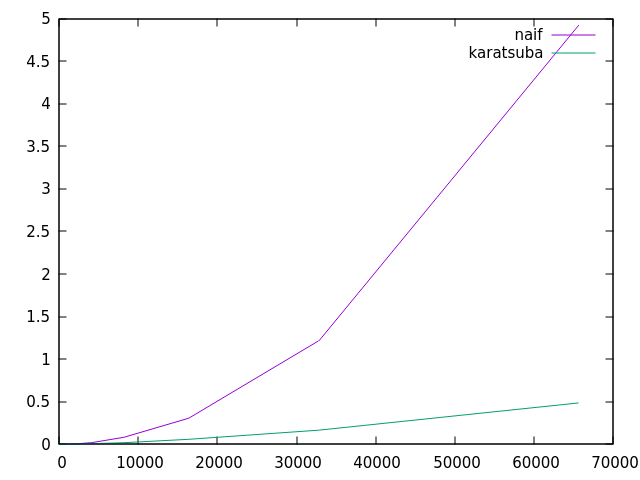
\includegraphics[scale=1]{naif_kara}\\


\section{Fast Fourier Transform (FFT)}

\newtheorem{Thm1}{Théorème}
\begin{Thm1}
Soient $a_1,\dots,a_n$ et $b_1,\dots,b_n$ des nombres réels (avec les $a_i$ deux à deux distincts). Aors il existe un unique polynôme P de degré n-1 tel que pour tout i dans $\{1,..., n\},\ P(a_i)\ =\ b_i$.
\end{Thm1}

La FFT se base sur ce théorème, en effet, l’idée est d’évaluer les polynômes $P$ et $Q$ en des points bien choisis, de faire le produits de ces évaluations et de retrouver l’unique polynôme $R=PQ$ à partir des valeurs du produit. Pour les points choisis, on prend les racines de l’unité car ?.
 
\begin{tcolorbox}[colback=cyan!5!white,
                  colframe=cyan!100!black,
                  title=\textbf{Algorithme FFT}
                 ]
\textbf{Entrée.} $P$ et $Q$ deux polynômes, n un entier, et $\omega$ une racine principale n-ième de l’unité. \\
\textbf{Sortie.} $R = PQ$ \\
\textbf{Algorithme.}
\begin{enumerate}[itemsep=-2ex]
\item\textit{Précalcul}. Calculer les puissances $\omega^2,\dots,\omega^{n-1}$. \\
\item\textit{Évaluation}. Calculer les valeurs : \\ $Eval(P)=(P(\omega^0),\dots,P(\omega^{n-1}))$ ; $Eval(Q)=(Q(\omega^0),\dots,Q(\omega^{n-1}))$. \\
\item\textit{Produit point à point}. $Eval(R) = (PQ(\omega^0),\dots,PQ(\omega^{n-1}))$. \\
\item\textit{Interpolation}. On retrouve $R$ grâce à $Eval(R)$.
\end{enumerate}
\end{tcolorbox}
On voit que la complexité des étapes de précalcul et de produit point à point sont en $O(n)$, le problème est désormais de voir comment effectuer les étapes d'évaluation de d'interpolation rapidement.

\subsection{Évalution d'un polynôme}
\subsubsection{Implémentation}
L'algorithme d'évaluation d'un polynôme est la deuxième étape de la FFT aussi appelé DFT (Discrete Fourier Transform), il se base sur le principe de diviser pour régner. 

\begin{tcolorbox}[colback=cyan!5!white,
                  colframe=cyan!100!black,
                  title=\textbf{Algorithme DFT}
                 ]
\textbf{Entrée.} \\
\textbf{Sortie.} \\
\textbf{Algorithme.}
\end{tcolorbox}

Soient $n = 2^k\ et\ P(X) = p_n X_n +\dots+p_1 X + p_0$, on note $P_0$ et $P_1$ les polynômes de coefficients respectivement pair et impair de $P$, c'est-à-dire :\\
$P_0(X) = p_{n} X^{n/2} +\dots+ p_2 X + p_0\ et\ P_1(X) = p_{n-1} X^{(n-1)/2} +\dots+ p_3 X + p_1$. \\
On a alors que $P(X) = P_0(X^2)+X P_1(X^2)$. \\
La DFT se base sur cette propriété.
...

\subsubsection{Tests de temps}
\begin{center}
\begin{tabular}{||c c c||}
\hline
Degré (+1) & Normal & AVX \\
\hline\hline
$2^{16}$ & 0 & XX \\
\hline
$2^{17}$ & 0 & XX \\
\hline
$2^{18}$ & 0.015625 & XX \\
\hline
$2^{19}$ & 0.031250 & XX \\
\hline
$2^{20}$ & 0.046875 & XX \\
\hline
$2^{21}$ & 0.125000 & XX \\
\hline
$2^{22}$ & 0.343750 & XX \\
\hline
$2^{23}$ & 0.812500 & XX \\
\hline
$2^{24}$ & 1.796875 & XX \\
\hline
\end{tabular}
\end{center}

\end{document}
